\chapter{Arduino Startup}
\chaplabel{arduino}

\section{Introduction}
This chapter gives the students an introduction to the hardware we are using and gets them started with 
the Arduino IDE.

\section{Datasheets}
\subsection{Arduino Nano Connect RP2040}
The data sheet for the Arduino Nano Connect RP2040 is located at\\ 
\href{https://docs.arduino.cc/resources/datasheets/ABX00053-datasheet.pdf}{https://docs.arduino.cc/resources/datasheets/ABX00053-datasheet.pdf}.

The main website for it is at \\
\href{https://docs.arduino.cc/hardware/nano-rp2040-connect}{https://docs.arduino.cc/hardware/nano-rp2040-connect}

The pinout is at \\
\href{https://content.arduino.cc/assets/Pinout\_NanoRP2040\_latest.png}{https://content.arduino.cc/assets/Pinout\_NanoRP2040\_latest.png}.

\subsection{RP2040 Microcontroller}
The RP2040 microcontroller datasheet (all 654 pages) is at \\
\href{https://datasheets.raspberrypi.com/rp2040/rp2040-datasheet.pdf}{https://datasheets.raspberrypi.com/rp2040/rp2040-datasheet.pdf}.

If you are ever interested in putting the microcontroller onto a circuit board yourself, there is a reference design at \\
\href{https://datasheets.raspberrypi.com/rp2040/hardware-design-with-rp2040.pdf}{https://datasheets.raspberrypi.com/rp2040/hardware-design-with-rp2040.pdf}.

\subsection{IMU - ST LSM6DSOXTR}
The IMU datasheet is at \\
\href{https://www.st.com/resource/en/datasheet/lsm6dsox.pdf}{https://www.st.com/resource/en/datasheet/lsm6dsox.pdf}

\subsection{Mic - ST MP34DT06JTR}
The microphone datasheet is at \\
\href{https://www.st.com/resource/en/datasheet/mp34dt06j.pdf}{https://www.st.com/resource/en/datasheet/mp34dt06j.pdf}

The \href{https://www.st.com/en/mems-and-sensors/mp34dt06j.html#sample-buy}{overview page} shows that the microphone is still actively being produced.

\subsection{WiFi and Bluetooth - U-blox® Nina W102}
The main page for the wireless unit is at \\
\href{https://www.u-blox.com/en/product/nina-w10-series-open-cpu}{https://www.u-blox.com/en/product/nina-w10-series-open-cpu}.

The datasheet is at \\
\href{https://www.u-blox.com/sites/default/files/NINA-W10\_DataSheet\_UBX-17065507.pdf}{https://www.u-blox.com/sites/default/files/NINA-W10\_DataSheet\_UBX-17065507.pdf}.

\subsection{Cryptographic IC - Microchip® ATECC608A}
Note that Microchip \href{https://www.microchip.com/en-us/product/ATECC608A}{doesn't suggest using this chip in new designs} so expect that some future versions of the
Nano RP2040 Connect to use the successor (\href{https://www.microchip.com/en-us/product/ATECC608B}{ATTECC608B}).

The datasheet for the A is here: \\
\href{https://ww1.microchip.com/downloads/en/DeviceDoc/ATECC608A-CryptoAuthentication-Device-Summary-Data-Sheet-DS40001977B.pdf}{https://ww1.microchip.com/downloads/en/DeviceDoc/ATECC608A-CryptoAuthentication-Device-Summary-Data-Sheet-DS40001977B.pdf}.

Note that it says it is a summary datasheet. You have to sign an NDA with Microchip to see the full datasheet.

\section{Installing the IDE}
These directions assume that you are using the lab computers and One Drive.
\begin{enumerate}
	\item Go to software download page: \href{https://www.arduino.cc/en/software}{https://www.arduino.cc/en/software}
	\item Download the Windows ZIP file (not the first link or the app)
	\item Open the zip file and copy the folder inside (arduino-1.8.19 as of this writing) into your One Drive folder. This may take a while. If you are on your own computer, you can use any of the programs.
	\item Once that transfer finishes, go into the folder and run arduino.exe. Windows will try to save you, but if you click More Info you can click Run Anyway.
	\item Windows Defender Firewall will also complain. Uncheck the box that is checked and/or click Cancel.
	\item It should load up with a window that looks like Figure \ref{fig:emptysketch}.
	\item In order to get it to connect correctly to your board, you need to install the Arduino Nano Connect RP2040 board.
	\begin{enumerate}
		\item Navigate to Tools$\rightarrow$Board: "Arduino Uno" (or similar)$\rightarrow$Boards Manager
		\item It should load as shown in Figure \ref{fig:boardsManager}.
		\item In the search bar, type "arduino nano connect" (without the quotes)
		\item The first item should be Arduino Mbed OS Nano Boards and should list the Arduino Nano RP2040 Connect.
		\item Move your cursor over it and it should show an Install button. Click it to install the board library.
		\item Wait for it to finish.
		\item While you are waiting, plug your Nano Connect into your computer and let it install it.
		\item As it finished, I received a User Account Control warning asking if I wanted to let dpinst-amd64.exe make changes to my device. I said yes.
		\item Next it asked me if I wanted to install Arduino Universal Serial Bus devices. Again, click to Install.
		\item It popped up again and I clicked Install again. Now it should say that the Arduino Mbed OS Nano Boards has been installed.
		\item Close the Boards Manager.
	\end{enumerate}
	\item Now go to Files$\rightarrow$Examples$\rightarrow$01.Basics$\rightarrow$Blink.
	\item This will open another window with the Blink program.
	\item Go to Tools$\rightarrow$Board$\rightarrow$Arduino Mbed OS Nano Boards and select the Arduino Nano RP2040 Connect
	\item Go to Tools$\rightarrow$Port and select the COM that isn't COM1 (mine showed up as COM5)
	\item Click the right arrow under the word edit in the menu to Uplaod the sketch to the Arduino board.
	\item It should say "Compiling sketch..." in the lower left and show a progress bar on the lower right.
	\item Then it should switch to Uploading... and finally Done Uploading.
	\item An orange light near the USB port on your board should be blinking.
	\item Congratulations! You have programmed your board!
	\item Now look in the program for the two delay statements. Try changing the values inside the parentheses and re-uploading it. Does the blinking change?
	\item In order to save files and have it portable, you need to change the directory where the Arduino IDE stores it's sketchbooks
	\begin{enumerate}
		\item Go to File$\rightarrow$Preferences
		\item Change the Sketchbook location to your OneDrive and a folder named arduino (lowercase is good)
		\item My OneDrive was in C:\textbackslash Users\textbackslash mcneils2\textbackslash OneDrive - Embry-Riddle Aeronautical University\textbackslash arduino
	\end{enumerate}
\end{enumerate}

\begin{figure}[!htb]
	\centering
	\includegraphics[scale=1.0]{arduinoStart/emptysketch.PNG}
	\caption{This is what the Arduino IDE should load up to.}
	\label{fig:emptysketch}
\end{figure} 

\begin{figure}[!htb]
	\centering
	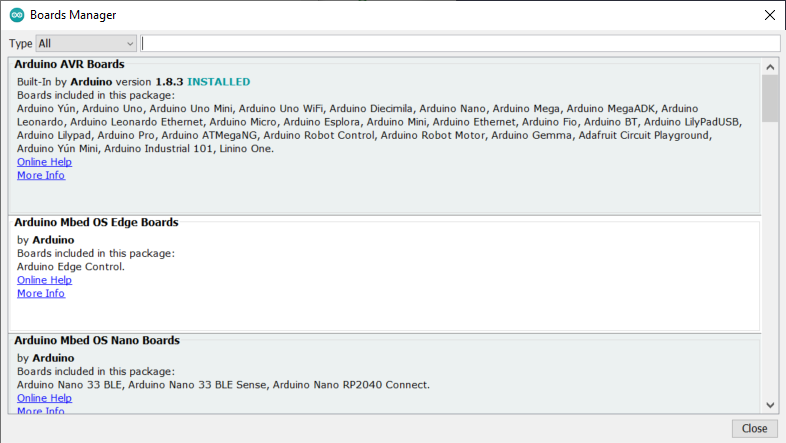
\includegraphics[scale=0.9]{arduinoStart/BoardsManager.PNG}
	\caption{This what the Boards Manager loads up to.}
	\label{fig:boardsManager}
\end{figure} 

\begin{figure}[!htb]
	\centering
	%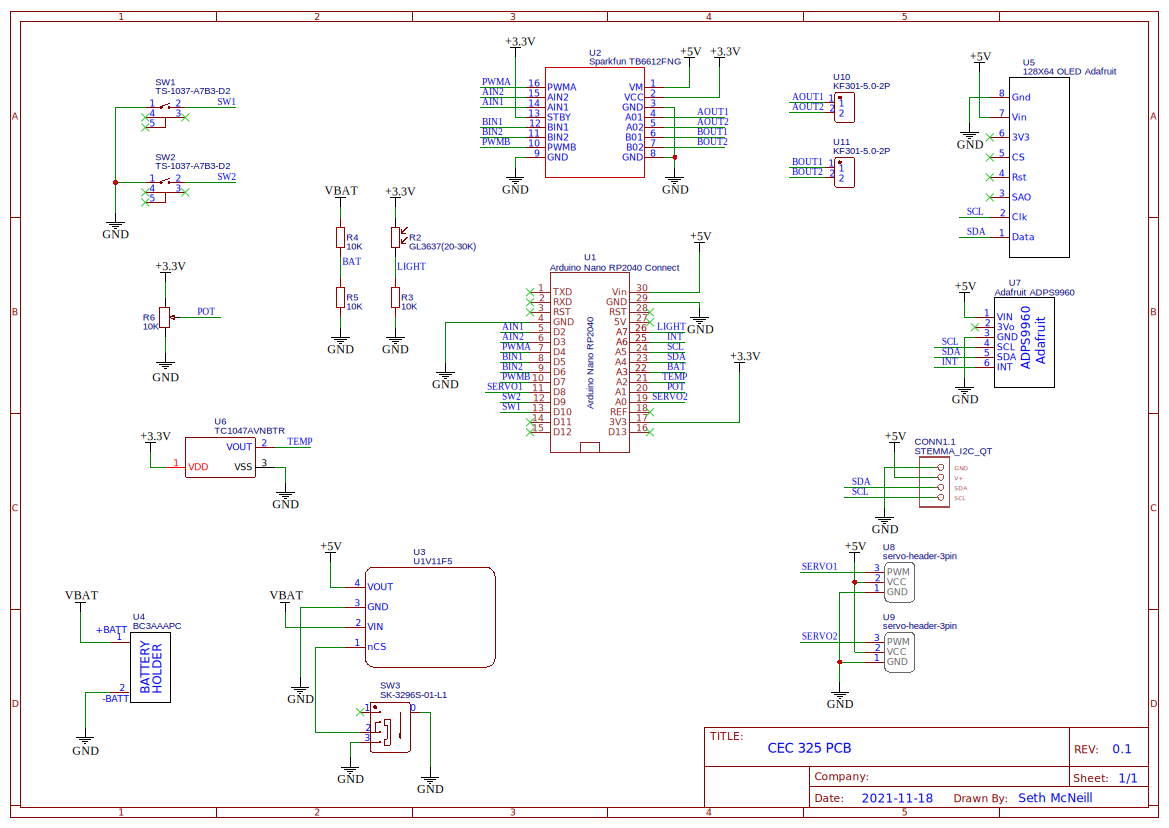
\includepdf[pages=-,pagecommand={},width=\textwidth]{arduinoStart/Schematic_NanoConnectRP2040test1_v0.1.pdf}
	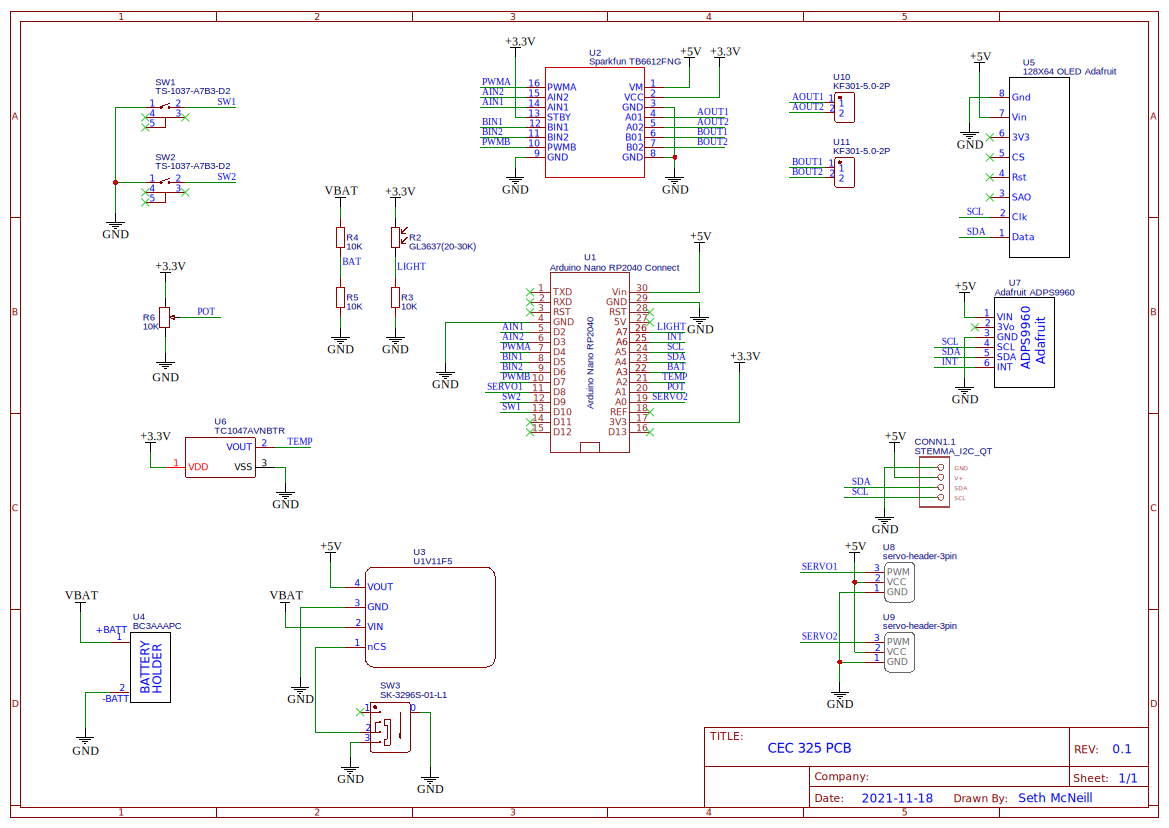
\includegraphics[width=\textwidth]{arduinoStart/Schematic_NanoConnectRP2040test1_v0.1} % leaving off extension seems to work
	\caption{This is the schematic of the first version of the board for the class.}
	\label{fig:boardSchematic}
\end{figure} 

\begin{figure}[!htb]
	\centering
	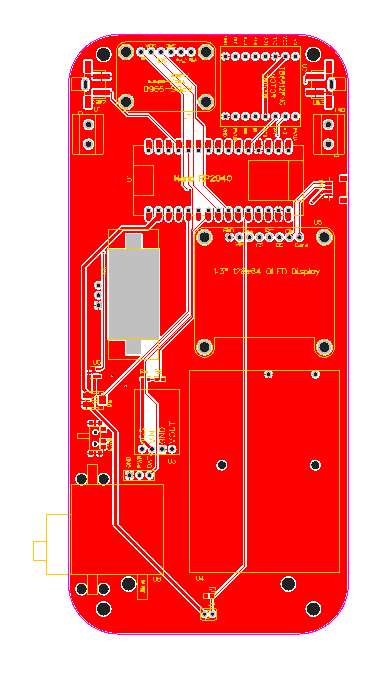
\includegraphics{arduinoStart/PCB_PCB_NanoConnectRP2040test1_v0.1} % leaving off extension seems to work
	\caption{This shows the top of the first version of the board for this class to help locate components.}
	\label{fig:boardTop}
\end{figure} 